\chapter{Validaci\'on de la Propuesta y Ejemplos de aplicaci\'on}

En los cap\'itulos anteriores de este documento hemos abordado el problema de la construcci\'on de \textit{APIs} de datos enlazados sem\'anticos desde la definici\'on de un modelo formal y un modelo arquitect\'onico hasta el dise\~no de componentes software que permitan implementar dicha arquitectura en una soluci\'on real.\\
En este cap\'itulo trataremos de mostrar la aplicabilidad de dicho modelo te\'orico y arquitect\'onico, as\'i como de los componentes software que hemos desarrollado para poder llevarlo a la pr\'actica. Para ello mostraremos los resultados obetnidos en la evaluaci\'on de rendimiento del componente clave par la construcci\'on de aplicaciones clientes que hemos desarrollado, el repositorio de tripletes RDF escrito en \textit{JavaScript}  y describiremos algunos ejemplos concretos que muestran c\'omo pueden ser usados para construir aplicaciones software que hacen uso de una \textit{API} de datos enlazados sem\'anticos para ofrecer nuevas soluciones a dominios de aplicaci\'on reales, como la construcci\'on de aplicaciones web sociales o la implementaci\'on de sistemas para visualizaci\'on de la informaci\'on en el navegador.\\
En todos los casos haremos un breve repaso de los problemas que el actual estado de implementaci\'on de este tipo de aplicaciones presenta para despu\'es centrarnos en qu\'e ventajas aporta el uso de datos enlazados sem\'anticos as\'i como en la implementaci\'on de dicha soluci\'on en el marco tecnol\'ogico propuesto anteriormente en este documento.

\section{Evaluaci\'on de rendimiento del Repositorio RDF para aplicaciones JavaScript}

En el cap\'itulo anterior (\ref{sec_rdfstorejs}) se describi\'o la implementaci\'on de un repositorio RDF \textit{SPARQL 1.1 Update} para aplicaciones \textit{JavaScript}.
Como parte final del proceso de desarrollo del repositorio, hemos realizado una evaluaci\'on de rendimiento de la biblioteca utilizando el modelo de evaluaci\'on \textit{LUBM} \cite{lubm} ajustado sus par\'ametros para usar un conjunto de datos peque\~no, m\'as adecuado al volumen de datos con el que debe tratar una aplicaci\'on web \textit{JavaScript}. La evaluaci\'on se ha realizado para diferentes navegadores web en un equipo port\'atil medio.\\
Los casos de prueba se han construido autom\'aticamente mediante el software generador de datos incluido dentro de \textit{LUBM} y a continuaci\'on se han transformado en \textit{JSON-LD} antes de ser cargados en el navegador para su ejecuci\'on. La cantidad final de tripletes almacenados en un \'unico grafo en el repositorio ha sido de 100.545 tripletes. La tabla \ref{tabla12} muestra los resultados obtenidos en milisegundos para las diferentes consultas \textit{LUBM}.\\

\begin{table}
\vspace{2.4in}
\centering
\caption{Pruebas de rendimiento \textit{LUBM} para el repositorio \textit{RDF}}
\vspace{5mm}
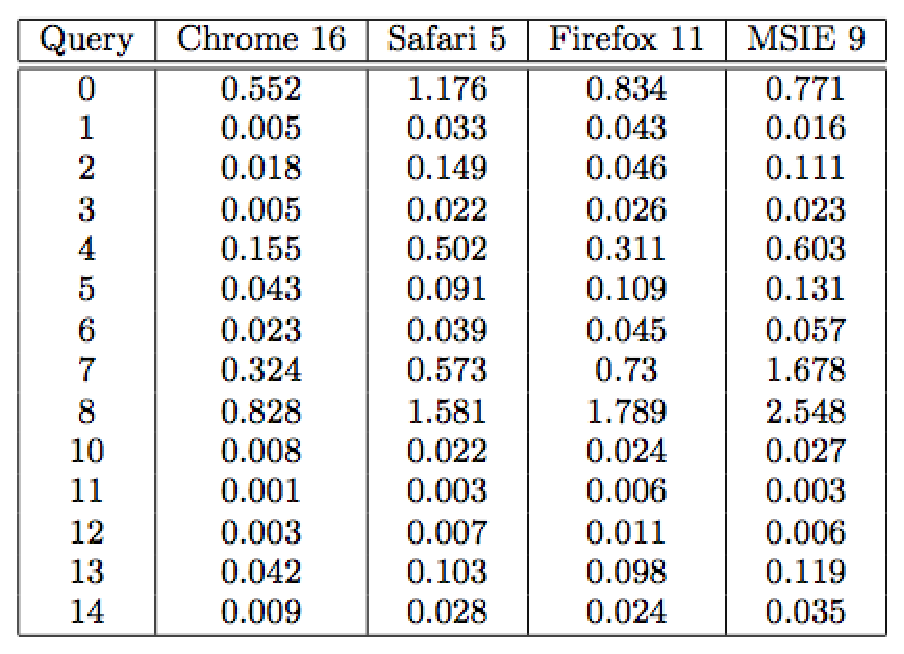
\includegraphics[width=0.8\textwidth]{tabla12}
\label{tabla12}
\end{table}

 Dado que el repositorio no soporta inferencia l\'ogica, algunas consultas en \textit{LUBM} han debido ser re-escritas para utilizar cl\'ausulas \textit{UNION} con el fin de cubrir todos los casos y obtener los resultados correctos esperados. Una consulta adicional que simplemente devuelve todos los tripletes ha sido tambi\'en a\~nadida. El texto de las consultas as\'i como el c\'odigo para ejecutar las consultas forma parte de la distribuci\'on de la biblioteca.
En los resultados se puede apreciar como la mayor\'ia de las consultas son evaluadas en un tiempo inferior al segundo. Siendo este el umbral m\'aximo de tiempo que consideramos aceptable para construir aplicaciones cliente que puedan ser utilizadas por el usuario final de una forma aceptable, adem\'as, el volumen de datos consultados y almacenados en el repositorio para las pruebas, es muy superior al volumen normal de tripletes que almacena una aplicaci\'on cliente de escritorio t\'ipica.
Realizando pruebas de carga con diferentes volumenes de datos, nos permite comprobar como el tiempo de las consultas se incrementa linealmente con el n\'umero de tripletes almacenados en el repositorio. Por \'ultimo, cabe destacar que un elemento decisivo para el rendimiento de la biblioteca es el motor \textit{JavaScript} del navegador web en el que se ejecuta la prueba. Diferentes navegadores con diferentes implementaciones de \textit{JavaScript} ofrecen rendimientos muy dispares para los mismos datos e implementaciones de la biblioteca. Esto puede suponer un problema a la hora de construir una aplicacion con un comportamiento predecible en diferentes plataformas. Por otro lado, el incremento en el rendimiento de los motores \textit{JavaScript} presentes en los actuales navegadores web es una de las principales preocupaciones de los fabricantes de dichos navegadores, con lo que es sensato esperar mejoras importantes en el rendimiento de estos motores y por lo tanto de la biblioteca y aplicaciones construidas sobre ella en el futuro cercano.


\section{Un servidor personal de datos enlazados sem\'anticos para la Web Social}

La Web Social est\'a compuesta hoy en d\'ia por un n\'umero ingente de diferentes servicios donde los usuarios mantienen fragmentos de su grafo social. La interoperabilidad entre diferentes redes sociales es un importante problema sin resolver en el dise\~no de la Web Social vigente hoy en d\'ia. Desde el punto de vista del acceso a los datos, la mayor\'ia de los sitios web sociales pueden considerarse silos de informaci\'on \cite{halpin2008beyond} donde la posibilidad de compartir datos a trav\'es aplicaciones se ve dificultada por mecanismos de autenticaci\'on, \textit{APIs}  y modelos de datos incompatibles.\\
La misma identidad de los usuarios tambi\'en se encuentra fragmentada entre aplicaciones. Diferentes mecanismos de autenticaci\'on y sistemas de credenciales son usadas para identificar al usuario en diferentes redes sociales. Como resultado, funcionalidades como la importaci\'on del grafo social de contactos de una red social d\'onde ya se es miembro a un nuevo servicio son tareas complejas que los usuarios deben completar antes de poder empezar a utilizar el nuevo servicio de una forma satisfactoria, convirti\'endose de esta manera en un importante barrera de entrada para la adopci\'on de nuevos servicios.\\
A pesar de los esfuerzos de estandarizaci\'on a los niveles de \textit{API} e identidad, como OAuth \cite{hammer2010oauth} y OpenID \cite{openid}, la tendencia reciente consiste en concentrar la autenticaci\'on de los usuarios en un peque\~no conjunto de proveedores de identidad como \textit{Google}, \textit{Twitter} o \textit{Facebook}. Una consecuencia de esta tendencia es que no s\'olo los datos sociales de los usuarios del servicio sino tambi\'en su mismas identidades son retenidos por un peque\~no conjunto de proveedores de servicios web, con el riesgo que esto supone de perdida de esa identidad si el servicio desaparece o la subordinaci\'on de los intereses del usuario a las pol\'iticas corporativas de dichas compa\~n\'ias.\\
En esta secci\'on describiremos c\'omo un servicio basado en una \textit{API} de datos enlazados sem\'anticos que hace uso de est\'andares desarrollados por las comunidades Web Sem\'antica y Datos Enlazados Abiertos en conjunci\'on con otras propuestas recientes aparecidas en el seno de dichas comunidades, como \textit{WebID}, puede ser una alternativa viable para la construcci\'on de redes sociales descentralizadas donde los usuarios tengan un mayor control sobre su identidad en la web y grafo social.\\
En concreto, el sistema descrito a continuaci\'on es capaz de recoger datos sociales de diferentes servicios en los que el usuario est\'a registrado, transformando todos estos datos diversos en un \'unico grafos social haciendo uso de un modelo de datos y una sem\'antica unificadas. El sistema asocia tambi\'en dicho grafo a una identidad \textit{WebID} para el usuario que puede ser generada y mantenida por el servicio o estar almacenada en cualquier otro proveedor \textit{WebID}.\\
El uso de tecnolog\'ias estandarizadas y abiertas hacen posible la integraci\'on el sistema como un nodo m\'as en una red social sem\'antica distribuida y desacoplada, introduciendo en dicha red los datos sociales ya existentes en otros servicios y ofreciendo al mismo tiempo la posibilidad de que las interacciones entre usuarios dentro de esta red puedan ser enviados de vuelta a redes sociales externas.

\subsection{Principios de dise\~no}

En el dise\~no del sistema, los siguientes principios b\'asicos fueron seguidos para intentar conseguir una aplicaci\'on que cumpliese con los objetivos de funcionalidad anteriormente propuestos:

\begin{itemize}
\item \textbf{Construcci\'on de un sistema extensible}, capaz de integrar datos de diferentes redes sociales ya existentes. Esto es posible gracias al dise\~no del sistema como un conjunto de extensiones para las diferentes redes sociales, capaces de captar informaci\'on proveniente de estas redes y traducirlas a datos \textit{RDF} usando una ontolog\'ia com\'un.  Vocabularios dentro de la comunidad Web Sem\'antica, especialmente dise\~nados para tratar con informaci\'on personal y social como SIOC \cite{sioc} y FOAF \cite{foaf} fueron usados con este fin.\\
\item \textbf{Exposici\'on de los datos a trav\'es de una \textit{API} \textit{REST}} construida siguiendo los principios formales y la arquitectura propuesta en este documento. Esto incluye la distinci\'on entre recurso \textit{HTTP} y recurso \textit{RDF} asociado, los mecanismos anteriormente explicados para generar \textit{URI} identificadores de los grafos asociados a los recursos o el uso de par\'ametros especiales para caracter\'isticas como la paginaci\'on.
\item \textbf{Uso de una identidad y autenticaci\'on distribuida basada en \textit{WebID}.} \textit{WebID} es un mecanismo de autenticaci\'on basado en el uso de \textit{URIs} y un empleo particular de la criptograf\'ia de clave p\'ublica. El resultado de desreferenciar una \textit{URI} asociada a una identidad \textit{WebID} no es s\'olo la informaci\'on de la clave p\'ublica necesario para validar la identidad del certificado autofirmado enviado por el cliente, sino un documento \textit{RDF} descrito usando el vocabulario \textit{FOAF} que incluye toda la informaci\'on de perfil (o enlaces a esa informaci\'on) que el due\~no de dicha identidad est\'e dispuesto a compartir p\'ublicamente. Esta informaci\'on es utilizada por el sistema para validar los derechos de acceso a los recursos expuestos examinando las relaciones de confianza establecidas entre el firmante de la petici\'on y el due\~no del recurso expuesto. El dise\~no de \textit{WebID} sigue los principios arquitect\'onicos \textit{REST}, con lo que ha sido muy f\'acil integrarlo en la arquitectura y modelo de servicios propuestos anteriormente en este documento.
\item \textbf{Capacidad para exponer datos sociales como objetos sociales} \cite{engestrom2005some}, \cite{engestrom1995voice}, que pueden ser definidos como entidades discretas de informaci\'on generadas por los usuarios de un servicio web social y que sirven como enlaces entre los usuarios de dicho servicio, proveyendo al mismo tiempo a esas interacciones de un contexto. Posts en un servicio de blogging o fotos en un servicio de fotograf\'ia social como \textit{Flickr}, son ejemplos de objetos sociales. Los objetos sociales son consumidos mediante un mecanismo de \textit{pull} donde los clientes usan el protocolo \textit{HTTP} para extraer una representaci\'on del objeto social expuesto como un recurso \textit{REST} sem\'antico \cite{kinsella2008navigating} y almacenado en el servicio como un peque\~no grafo \textit{RDF} denominado \textit{mol\'ecula RDF} \cite{ding2005tracking}. 
\textit{Capacidad para exponer datos sociales como un flujo social}, que puede ser definido como una colecci\'on ilimitada de datos sociales con una dimensi\'on temporal y una identidad estable asociadas. Servicios de estado social como \textit{Twitter} son ejemplos de este tipo de datos sociales. El uso que de este tipo de datos sociales hacen los usuarios es t\'ipicamente \textit{push} donde es el servicio el que notifica al cliente sobre nuevos eventos en el flujo. 
\end{itemize}

\subsection{Arquitectura del sistema}

La arquitectura del sistema se basa en el modelo arquitect\'onico expuesto en secciones anteriores de este documento. En este apartado expondremos las principales extensiones que de dicho modelo se han llevado a cabo con el fin de publicar los diferentes tipos de datos sociales que se pretend\'ian compartir. La figura \ref{figura5} muestra el flujo de informaci\'on a trav\'es de los principales componentes del sistema.\\

\begin{figure}
\centering
\caption{Flujo de informaci\'on en el sistema.}
\vspace{5mm}
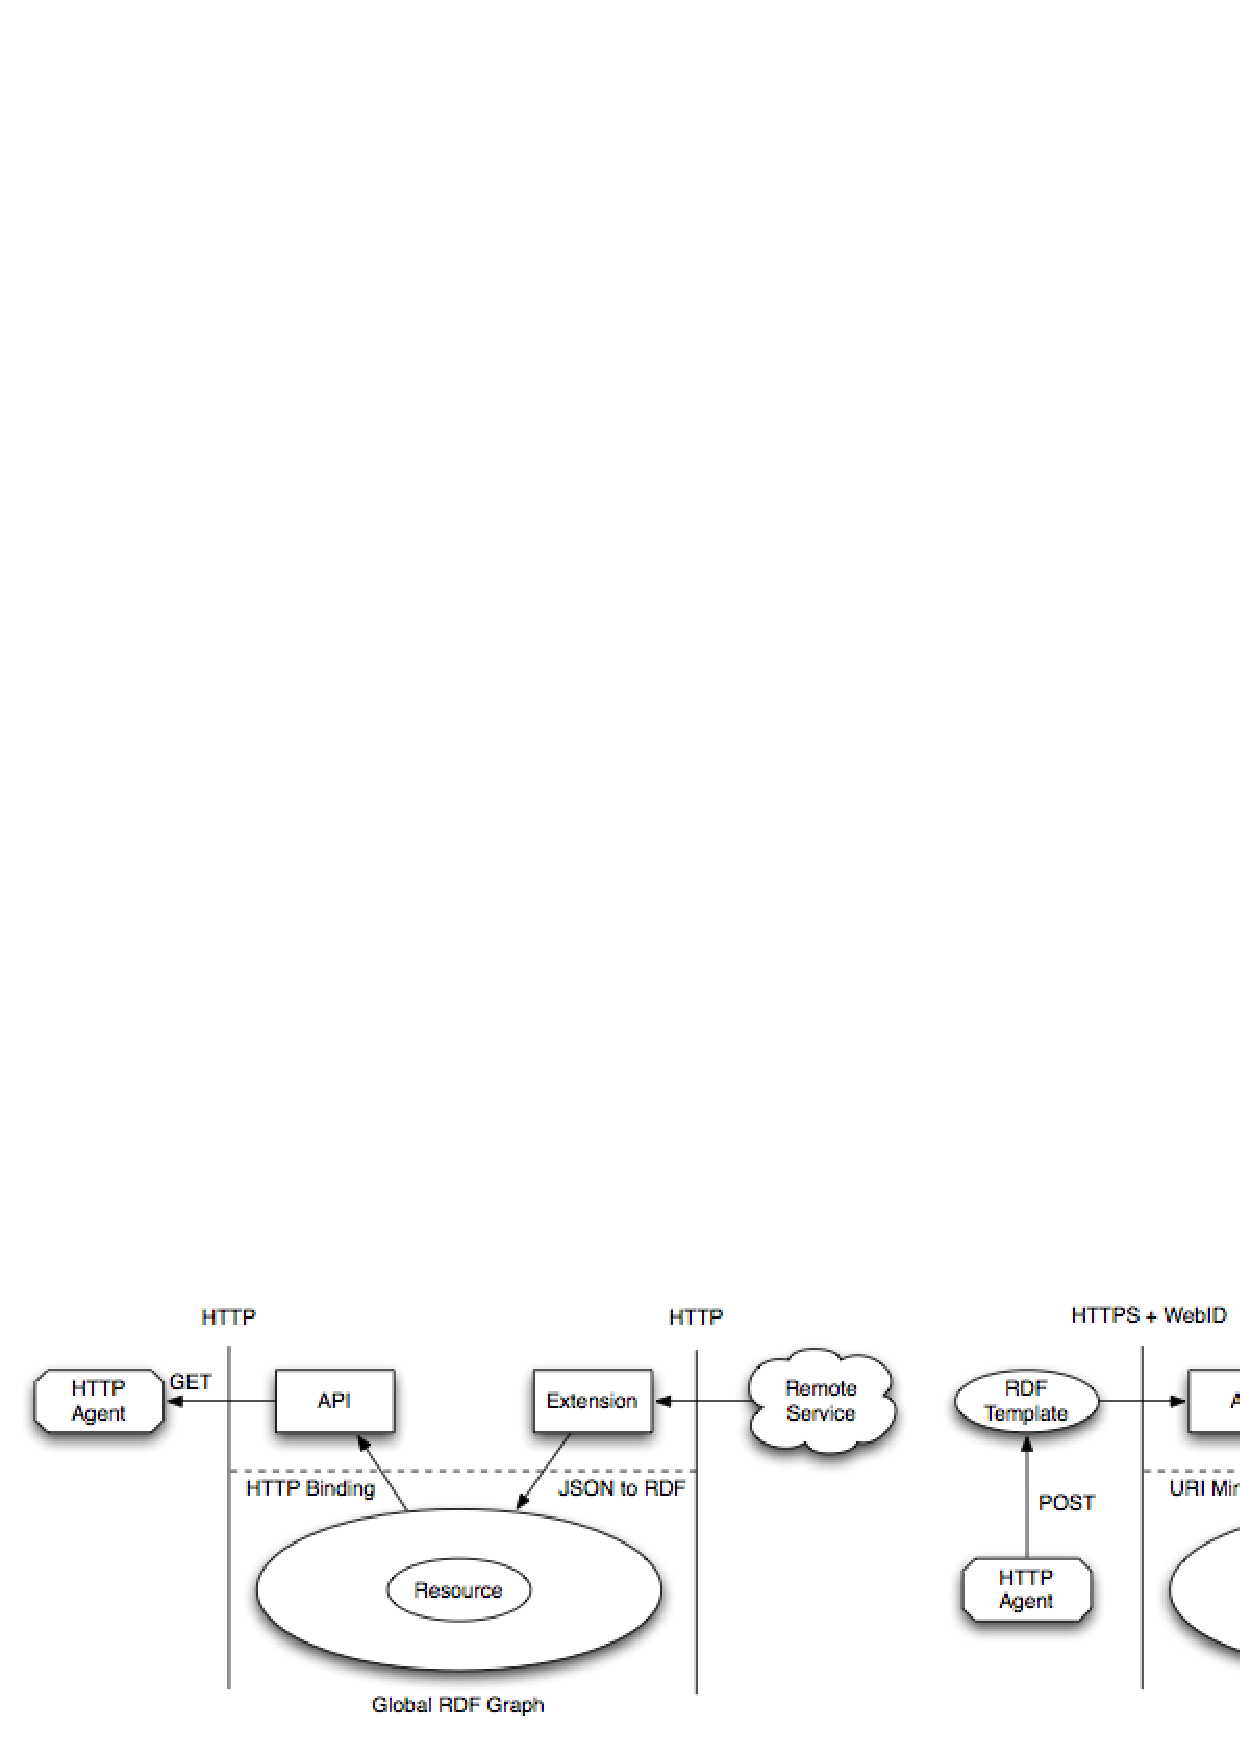
\includegraphics[width=1\textwidth]{figura5}
\label{figura5}
\end{figure}


\begin{itemize}
\item \textbf{Concepci\'on de la aplicaci\'on como un sistema modular.} Cada m\'odulo gestiona la interacci\'on con una red social diferente y se ejecutan de una forma completamente aut\'onoma cooperando a trav\'es del uso de un mecanismos de mensajes y de una ontolog\'ia \textit{RDF} com\'un donde se exponen los tipos de recursos que la extensi\'on va a generar. Gracias a este vocabulario com\'un, el n\'ucleo de la aplicaci\'on es capaz de integrar esos recurso en la \textit{API} \textit{HTTP}, recuperarlos del repositorio \textit{RDF} y darles el formato adecuado si es necesario.
\item \textbf{Integraci\'on de la autenticaci\'on \textit{WebID}.} En la definici\'on de la arquitectura de servicios \textit{REST} sem\'anticos expuesta anteriormente no se mencionaron los aspectos de seguridad relativos a la autenticaci\'on del acceso a los recursos expuestos. La aplicaci\'on construida soluciona este problema mediante el uso de \textit{WebID}. Cualquier recurso expuesto a trav\'es de la \textit{API}, puede ser marcado como publico, privado o accesible s\'olo por un determinado n\'umero de identidades \textit{WebID}. El sistema se encarga de autenticar la identidad de los usuarios accediendo a los recursos remotos con informaci\'on sobre la identidad del cliente en cada petici\'on \textit{HTTP} realizando el proceso de autenticaci\'on \textit{WebID} y comprobando el grafo \textit{RDF} resultante de a\~nadir la informaci\'on del perfil remoto obtenida con los datos de perfil de usuario mantenidos localmente. Este proceso es completamente \textit{REST} involucrando simplemente la desrefernciaci\'on de la \textit{URI} asociada a la identidad del cliente y la comprobaci\'on criptogr\'afica de su veracidad.
\item \textbf{Exposici\'on de un flujo social de datos.} El concepto de flujo social se traduce mal en t\'erminos \textit{REST} tanto por su naturaleza no discreta y din\'amica, como por el hecho de estar pensado para ser consumido mediante un mecanismo \textit{push} en el que el servicio notifica a los clientes de la presencia de nuevos datos. En nuestra implementaci\'on hemos optado por una opci\'on intermedia en el que el consumo del flujo es todav\'ia \textit{pull} siendo los clientes los encargados de realizar alg\'un tipo de petici\'on peri\'odica para obtener los nuevos eventos expuestos. Para ello, el flujo se asocia a una \textit{URI} estable y bien conocida, donde los clientes pueden realizar peticiones de solo lectura mediante operaciones \textit{GET} \textit{HTTP}. Las diferentes extensiones aut\'onomas de la aplicaci\'on pueden publicar en cualquier momento informaci\'on en el flujo insertando en el grafo recursos \textit{RDF} con un tipo \textit{SIOC} \textit{MicroBlogPost}.
\item \textbf{Implementaci\'on de \textit{SPARQL} WebHooks}. Para mitigar el problema del consumo del flujo de datos mediante peticiones peri\'odicas, el sistema tambi\'en emplea un sistema que permite a un cliente con una \textit{URI} desreferenciable e identificado por una identidad \textit{WebID} crear una petici\'on de notificaci\'on web (\textit{WebHook}) con una consulta \textit{SPARQL} asociada. Si una modificaci\'on del grafo de la aplicaci\'on resulta en una respuesta satisfactoria de la consulta \textit{SPARQL}, los resultados ser\'an enviadas a la \textit{URI} provista por la identidad \textit{WebID} que creo la petici\'on de notificaci\'on en el sistema. Las peticiones de notificaci\'on se exponen en el sistema como otro recurso sem\'antico m\'as con la excepci\'on de que puedenser manipuladas, no solo por el administrador del servicio, sino por los clientes remotos que crearon dichas peticiones de notificaci\'on.
\end{itemize}

\subsection{Detalles de implementaci\'on}

El prototipo del sistema aqu\'i detallado fue implementado usando la plataforma de desarrollo de aplicaciones \textit{JavaScript} \textit{Node.JS}. La capa de persistencia \textit{RDF} se implement\'o usando la base de datos no relacional \textit{MongoDB}, d\'onde se almacenaron las \textit{mol\'ecula}s \textit{RDF} directamente como objetos \textit{JSON-LD}. Los componentes para llevar a cabo la generaci\'on de identidades \textit{WebID} o llevar a cabo la autenticaci\'on tambi\'en fueron desarrollados como bibliotecas para \textit{Node.JS} y liberados posteriormente con licencia de C\'odigo Abierto.\\
En aquellos momentos en el que la ejecuci\'on de consultas \textit{SPARQL} resultaba indispensable, nuestra propia librer\'ia que implementa un repositorio \textit{RDF} \textit{JavaScript} con soporte para \textit{SPARQL 1.1 Update} fue utilizada, cargando en el repositorio los documentos \textit{JSON-LD} recuperados desde \textit{MongoDB} que son necesarios.
Como parte de la implementaci\'on del sistema, componentes modulares para los servicios de web sociales \textit{Twitter}, \textit{Github} y un componente gen\'erico para feeds \textit{RSS/Atom} fueron desarrollados.\\
La \textit{API} \textit{HTTP} expuesta soporta peticiones procedentes de clientes \textit{JavaScript} ejecut\'andose en el navegador desde dominios diferentes a los del servicio gracias a la implementaci\'on del est\'andar de peticiones \textit{cross domain} (\textit{CORS}) \cite{cors} de la \textit{W3C}.\\
Por \'ultimo, algunas aplicaciones clientes \textit{JavaScript} han sido desarrollados e incluidas en el sistema para consumir la \textit{API} que el servicio expone. Una primera aplicaci\'on administrativa accede a los recursos de perfil y configuraci\'on de la \textit{API} para configurar la informaci\'on de perfil del usuario del servicio as\'i, como las pol\'iticas de acceso a los recursos expuestos y de gesti\'on de la identidad \textit{WebID} del usuario.\\
La figura \ref{figura6} muestra el aspecto de otra de las aplicaciones incluidas capaz de visualizar el flujo social de una identidad \textit{WebID} alojada en el servicio. Se puede observar como notificaciones generadas por diferentes componentes (Twitter, Github) se mezclan en el flujo social del usuario. \\

\begin{figure}
\vspace{2.4in}
\centering
\caption{Aplicaci\'on \textit{JavaScript} mostrando el flujo de actividad de un usuario.}
\vspace{5mm}
\includegraphics[width=1\textwidth]{screenshot}
\label{figura6}
\end{figure}


Ambas aplicaciones usan nuestro repositorio \textit{RDF} \textit{JavaScript} ejecut\'andose en el navegador para agregar los recursos \textit{REST} sem\'anticos expuestos a trav\'es de la \textit{API} de datos enlazados sem\'anticos y construir con ellos una p\'agina final \textit{HTML} que tambi\'en incorpora la informaci\'on \textit{RDF} extra\'ida mediante el uso del est\'andar \textit{RDFa}.

\section{Visualizaci\'on de datos \textit{RDF} en aplicaciones \textit{JavaScript}}

En el caso de aplicaci\'on anterior, hemos visto como el uso de una \textit{API} de datos enlazados sem\'anticos hace posible transformar el dise\~no y las caracter\'isticas de un dominio de aplicaci\'on especifico, como es el caso de la construcci\'on de redes sociales de usuarios. En esta secci\'on nos centraremos en un caso de aplicaci\'on m\'as concreto, como es el de la construcci\'on de visualizaciones de datos en un cliente \textit{JavaScript} ejecut\'andose en el navegador, para intentar mostrar como el uso de informaci\'on sem\'antica disponible en una \textit{API} enlazada sem\'antica y el uso de librer\'ias espec\'ificas que hagan su tratamiento sencillo, como el repositorio \textit{RDF} \textit{JavaScript} que hemos descrito en secciones anteriores, permite ofrecer soluciones alternativas m\'as simples en este dominio de aplicaci\'on.\\
Generar visualizaciones de datos a partir de grafos \textit{RDF}, especialmente usando \textit{JavaScript} en el navegador es un proceso complejo y tedioso. La dificultad radica en el hecho de que las bibliotecas de visualizaci\'on de datos disponibles, como \textit{D3} \cite{d3}, no est\'an preparadas para trabajar directamente con el modelo de datos \textit{RDF}, necesit\'andose por tanto, un proceso de limpieza y transformaci\'on de los datos en el modelo de datos que la biblioteca demanda para cada tipo de visualizaci\'on en concreto, problema que se vuelve todav\'ia m\'as compleja si se intenta combinar en la visualizaci\'on diferentes fuentes de datos de varios proveedores.\\
En esta secci\'on describmos una biblioteca \textit{JavaScript} para la construcci\'on de visualizaciones de datos, que tiene en cuenta las caracter\'isticas del modelo de datos \textit{RDF} para definir la visualizaci\'on. El sistema se ha construido sobre la biblioteca que implementa un repositorio \textit{RDF} para \textit{JavaScript} con soporte para consultas \textit{SPARQL 1.1 Update} que describimos en secciones anteriores.

\subsection{Gram\'atica de gr\'aficos para \textit{RDF}}

La biblioteca se ha construido sobre las ideas de una gram\'atica de gr\'aficos \cite{wilkinson2012grammar}, un conjunto finito de operaciones de alto nivel que se pueden combinar de diferentes maneras para generar un numero determinado visualizaciones gr\'aficas, dados unos datos iniciales de entrada.\\
La biblioteca construida extiende las operaciones cl\'asicas de este tipo de gram\'aticas de gr\'aficos,  con dos operaciones espec\'ificas para manipular datos \textit{RDF}:

\begin{itemize}
\item \textbf{Selecci\'on de datos \textit{RDF}}, mediante consultas \textit{SPARQL} y la selecci\'on de una estructura de datos de destino: lista, \'arbol o grafo, donde los nodos \textit{RDF} seleccionados ser\'an autom\'aticamente coercionados.
\item \textbf{\textit{Join} de datos generalizado}. Mediante el cual los nodos \textit{RDF} recuperados e introducidos en la estructura de datos seleccionada, son asociados a marcas visuales en la visualizaci\'on, traduci\'endose durante el proceso las propiedades \textit{RDF} del recurso en caracter\'isticas visuales de la marca visual asociada, como la posici\'on, el radio, la altura y anchura, el color, etc.
\end{itemize}

La tabla \ref{tabla13} muestra la sintaxis final de la biblioteca, mostrando como el vocabulario de la gram\'atica puede usarse para construir una visualizaci\'on. La figura \ref{figura7} muestra el resultado final de esa misma descripci\'on.\\

\begin{table}
\vspace{2.4in}
\caption{Definici\'on de una visualizaci\'on usando la gram\'atica de gr\'aficos.}
\vspace{5mm}
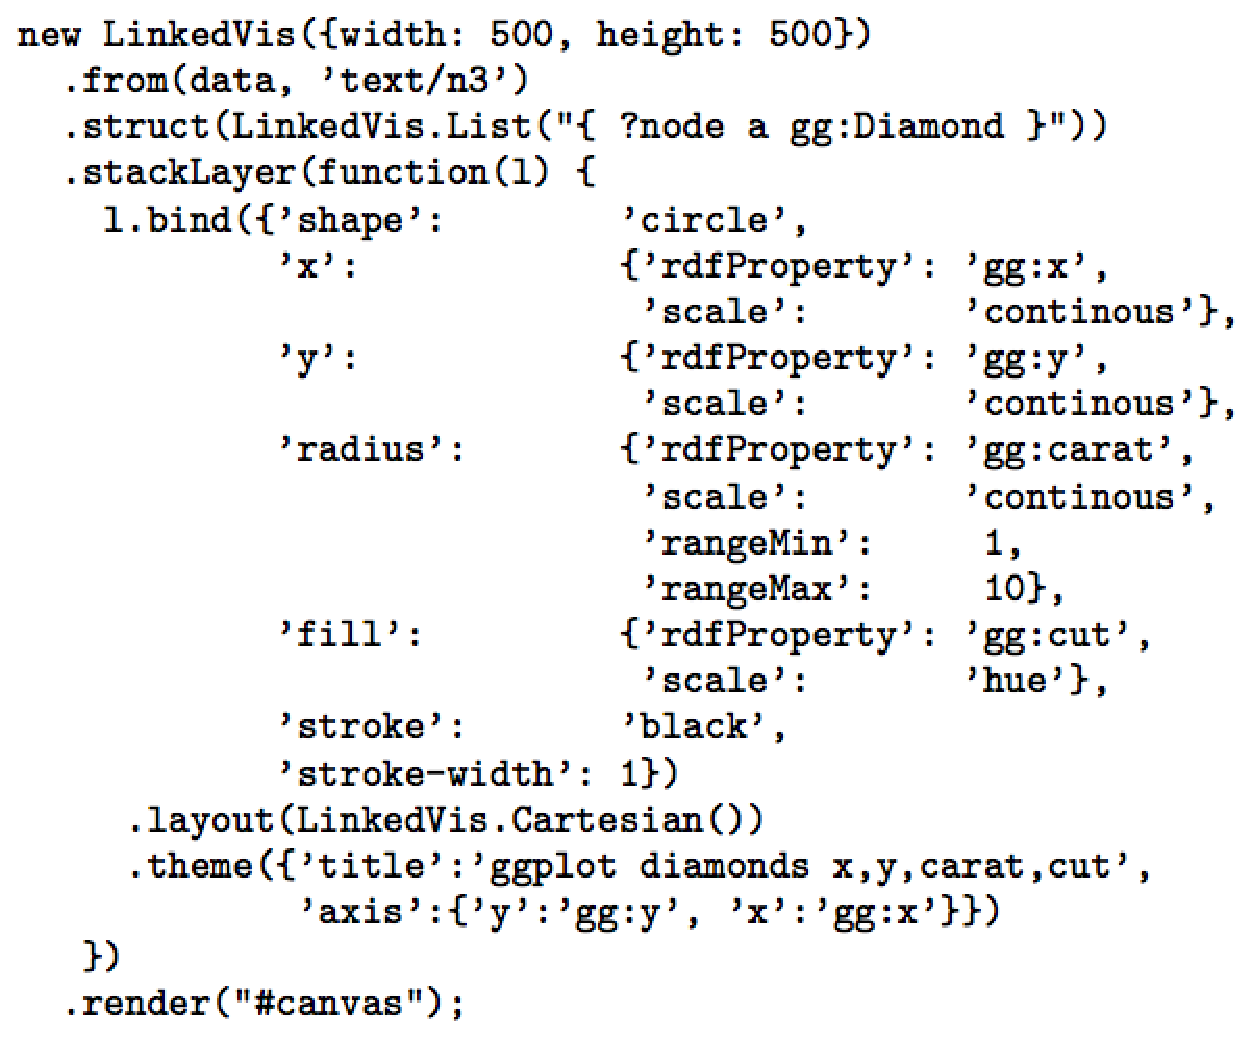
\includegraphics[width=0.8\textwidth]{tabla13}
\label{tabla13}
\end{table}

\begin{figure}
\vspace{2.4in}
\centering
\caption{Visualizaci\'on generada por la biblioteca a partir del c\'odigo de la tabla \ref{tabla13}}
\vspace{5mm}
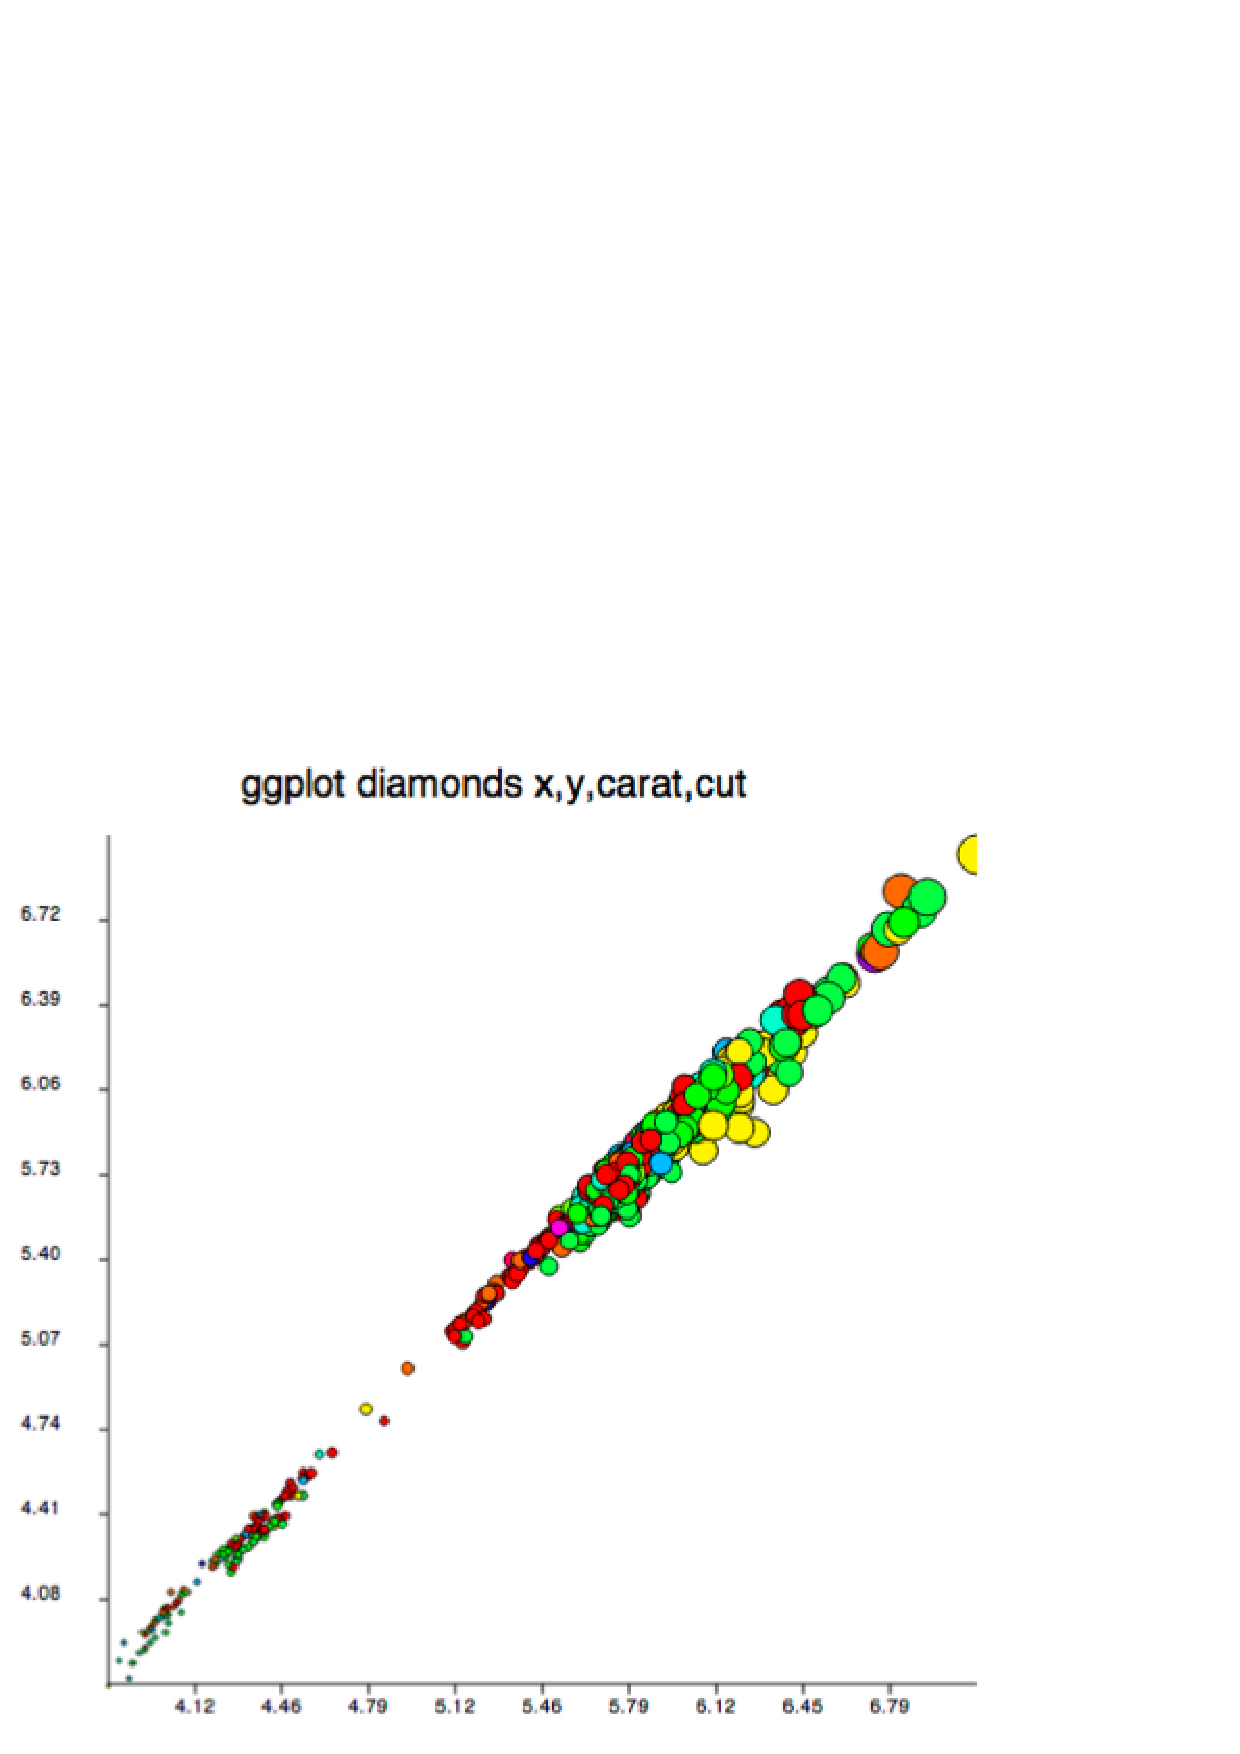
\includegraphics[width=0.8\textwidth]{figura7}
\label{figura7}
\end{figure}

Se puede observar como la funci\'on \textit{struct} introduce una estructura de datos de destino para los nodos \textit{RDF} recuperados por una consulta \textit{SPARQL}. A su vez, la funci\'on \textit{bind} realiza el \textit{join} entre datos y marcas visuales, usando para ello las propiedades \textit{RDF} de los nodos recuperados que son asignadas a diferentes valores de las propiedades de la marca.

\subsection{Dise\~no e implementaci\'on}

El dise\~no de la biblioteca se basa en la ejecuci\'on de cuatro etapas que conducen a la generaci\'on de la visualizaci\'on final como un documento \textit{SVG} insertado en el \'arbol \textit{DOM} de la p\'agina \textit{HTML} de destino.

\begin{itemize}
\item \textbf{Selecci\'on de datos}. Es el proceso por el que el usuario de la gram\'atica selecciona el origen de los datos \textit{RDF}, un recurso \textit{REST} sem\'antico remoto, el texto de un documento \textit{RDF} o una instancia del objeto repositorio \textit{RDF}, y lo transforma en una estructura de destina mediante una consulta \textit{SPARQL}. La biblioteca soporta tres diferentes estructuras de datos de desitno, listas, \'arboles y grafos. Cada una de estas estructuras requieren que el usuario especifique consultas \textit{SPARQL} con cierta estructura, usando valores espec\'ificos de las variables \textit{SPARQL} que luego ser\'an utilizados por la l\'ogica de la estructura de datos de destino para recuperar los datos.
\item \textbf{Composici\'on de capas}. La visualizaci\'on es construida por la biblioteca como un conjunto de capas que pueden ser superpuestas, compartiendo entonces los mismos l\'imites que la capa inferior,  o anidadas dentro de otra, con lo que la nueva capa queda restringida a un sub\'area de la capa padre. La capa recibe la selecci\'on de datos actual que ser\'a usada para generar las marcas visuales necesarias dentro de la capa.
\item \textbf{\textit{join} de marcas visuales}. Dentro de una capa, es posible realizar una operaci\'on de \textit{join} entre  los datos de la selecci\'on anterior y un tipo de marca visual con determinadas propiedades est\'eticas. La biblioteca soporta diferentes tipos de marcas, entre las que algunas coinciden con elementos \textit{SVG}, como \textit{rect}, \textit{circle} o \textit{text}. Las propiedades est\'eticas de cada marca se asocian a las propiedades \textit{RDF} del nodo \textit{RDF} que ha sido asignado a la marca mediante la operaci\'on de \textit{join}. Las propiedades est\'eticas se pueden clasificar en propiedades dimensi\'on, como la posici\'on \textit{x}, \textit{y}, el radio, etc, propiedades de estilo, modeladas de acuerdo a las propiedades \textit{CSS} como el color de relleno o el color de trazo y por \'ultimo, propiedades espec\'ificas para el tipo de layout que se ha asignado a la capa, como veremos a continuaci\'on. Los valores de estas propiedades est\'eticas se pueden especificar como un valor constante, el valor de la propiedad \textit{RDF} asociada o una funci\'on de escala que toma como valor de entrada el valor de la propiedad \textit{RDF}.
\item \textbf{Procesamiento del layout}. Cada capa de la visualizaci\'on debe declarar una propiedad de \textit{layout}, usada por la biblioteca para computar la posici\'on de cada marca visual en la visualizaci\'on. Para ello el \textit{layout} utilizar\'a el valor de las propiedades est\'eticas de cada marca visual. Los \textit{layouts} soportados por la biblioteca se organizan de forma jer\'arquica, siendo los \textit{layouts} \textit{cartesiano} y \textit{polar} los m\'as gen\'ericos. Distintos \textit{layouts} generan diferentes visualizaciones y exigen diferentes propiedades en las marcas visuales.
\end{itemize}

\subsection{Visualizaciones enlazadas}

Una de las funcionalidades de la biblioteca construida que no suele estar presente en otras soluciones para la generaci\'on de visualizaciones de datos es el de la inclusi\'on de abundantes meta-datos \textit{RDF} en la propia visualizaci\'on. Estos es posible gracias a que el formato \'ultimo de la visualizaci\'on generada consiste en un documento SVG con formato \textit{XML}. Dos grafos est\'an presentes en la visualizaci\'on final generada.

\begin{itemize}
\item \textbf{Grafo de datos}. Es un grafo \textit{RDF} conteniendo la agregaci\'on de todos los nodos \textit{RDF} seleccionados en todas las capas de la visualizaci\'on.
\item \textbf{Meta-grafo}. Conteniendo una descripci\'on de la visualizaci\'on usando una ontolog\'ia espec\'ifica. Este grafo incluye detalles como el n\'umero de capas, las estructuras de datos usadas o qu\'e nodos del grafo de datos est\'an asociados a qu\'e marcas visuales.
\end{itemize}

La presencia de ambos tipos de grafos abre la puerta a la construcci\'on de bibliotecas capaz de manipular la visualizaci\'on en funci\'on de la descripci\'on de la misma que se encuentra insertada en ella para a\~nadir un elemento de interactividad al uso que de la visualizaci\'on har\'an los usuarios finales. La generaci\'on de ambos grafos de meta-datos es opcional y puede ser desactivada.